\section{问题四：波动电价下的策略比较}
\subsection{价格信息与模型修正}
将固定分时电价$p_t$推广为目标日期的$p_{d,t}$。附件4价格曲线作为给定条件输入，而负载、光伏仍保持原有信息约束。365天日期与144个时间列严格与附件2对齐；1月价格不计入334天正式结果。若未来价格未知，则需另建预测或随机价格场景，超出当前基础方案。

问题4-2将第二问目标改为$\sum_tp_{d,t}G_t+\sum_s\pi_s\sum_t5p_{d,t}U_t^{(s)}+\varepsilon\sum_t(C_t+D_t)$，其他约束不变。问题4-3同样替换初始计划、紧急补购与调整交易的价格：
\begin{equation}K_d^r=\sum_{t\in\mathcal T_r}p_{d,t}(1.5A_t^r-0.5B_t^r).\end{equation}
历史窗口、中点插值、设备参数及每日边界均保持一致，正式4-3继续采用0、6、12点策略。固定价格基线使用同一策略，避免把更新时间变化混入价格机制比较。
\subsection{年度结果与经济机制}

\begin{table}[H]\centering\small
\caption{固定与波动价格下的334天对比}
\begin{tabular}{lrrr}\toprule
策略 & 总费用/元 & 紧急电量/kWh & 紧急费/元\\\midrule
问题二 & 17609791.6865 & 477446.0574 & 1837978.9991\\
问题4-2 & 17923538.0937 & 476815.3372 & 2115778.9637\\
问题三 & 17020306.6465 & 282085.6383 & 1077450.6027\\
问题4-3 & 17244554.4259 & 281004.2788 & 1214613.7429\\
\bottomrule\end{tabular}\end{table}
波动价格下，日前策略费用增加313746.4071元（1.7817\%），滚动策略增加224247.7793元（1.3175\%）。在相同波动价格环境中，4-3比4-2节省678983.6678元，降幅3.7882\%。该差异体现新增预报、场景构造及滚动交易的综合价值。
两组动态策略的紧急电量略低于固定价格基线，但紧急费用更高，说明缺口出现在哪个价格时段同样重要。平均电价降低也不能保证总费用降低，因为费用取决于购电量与逐时价格的配对及五倍补购。充放电时移还受到0.81往返效率约束；简化的无其他约束套利条件为高价超过低价的$1/0.81$倍，完整模型还需计入供能风险与容量机会成本。

\begin{figure}[H]\centering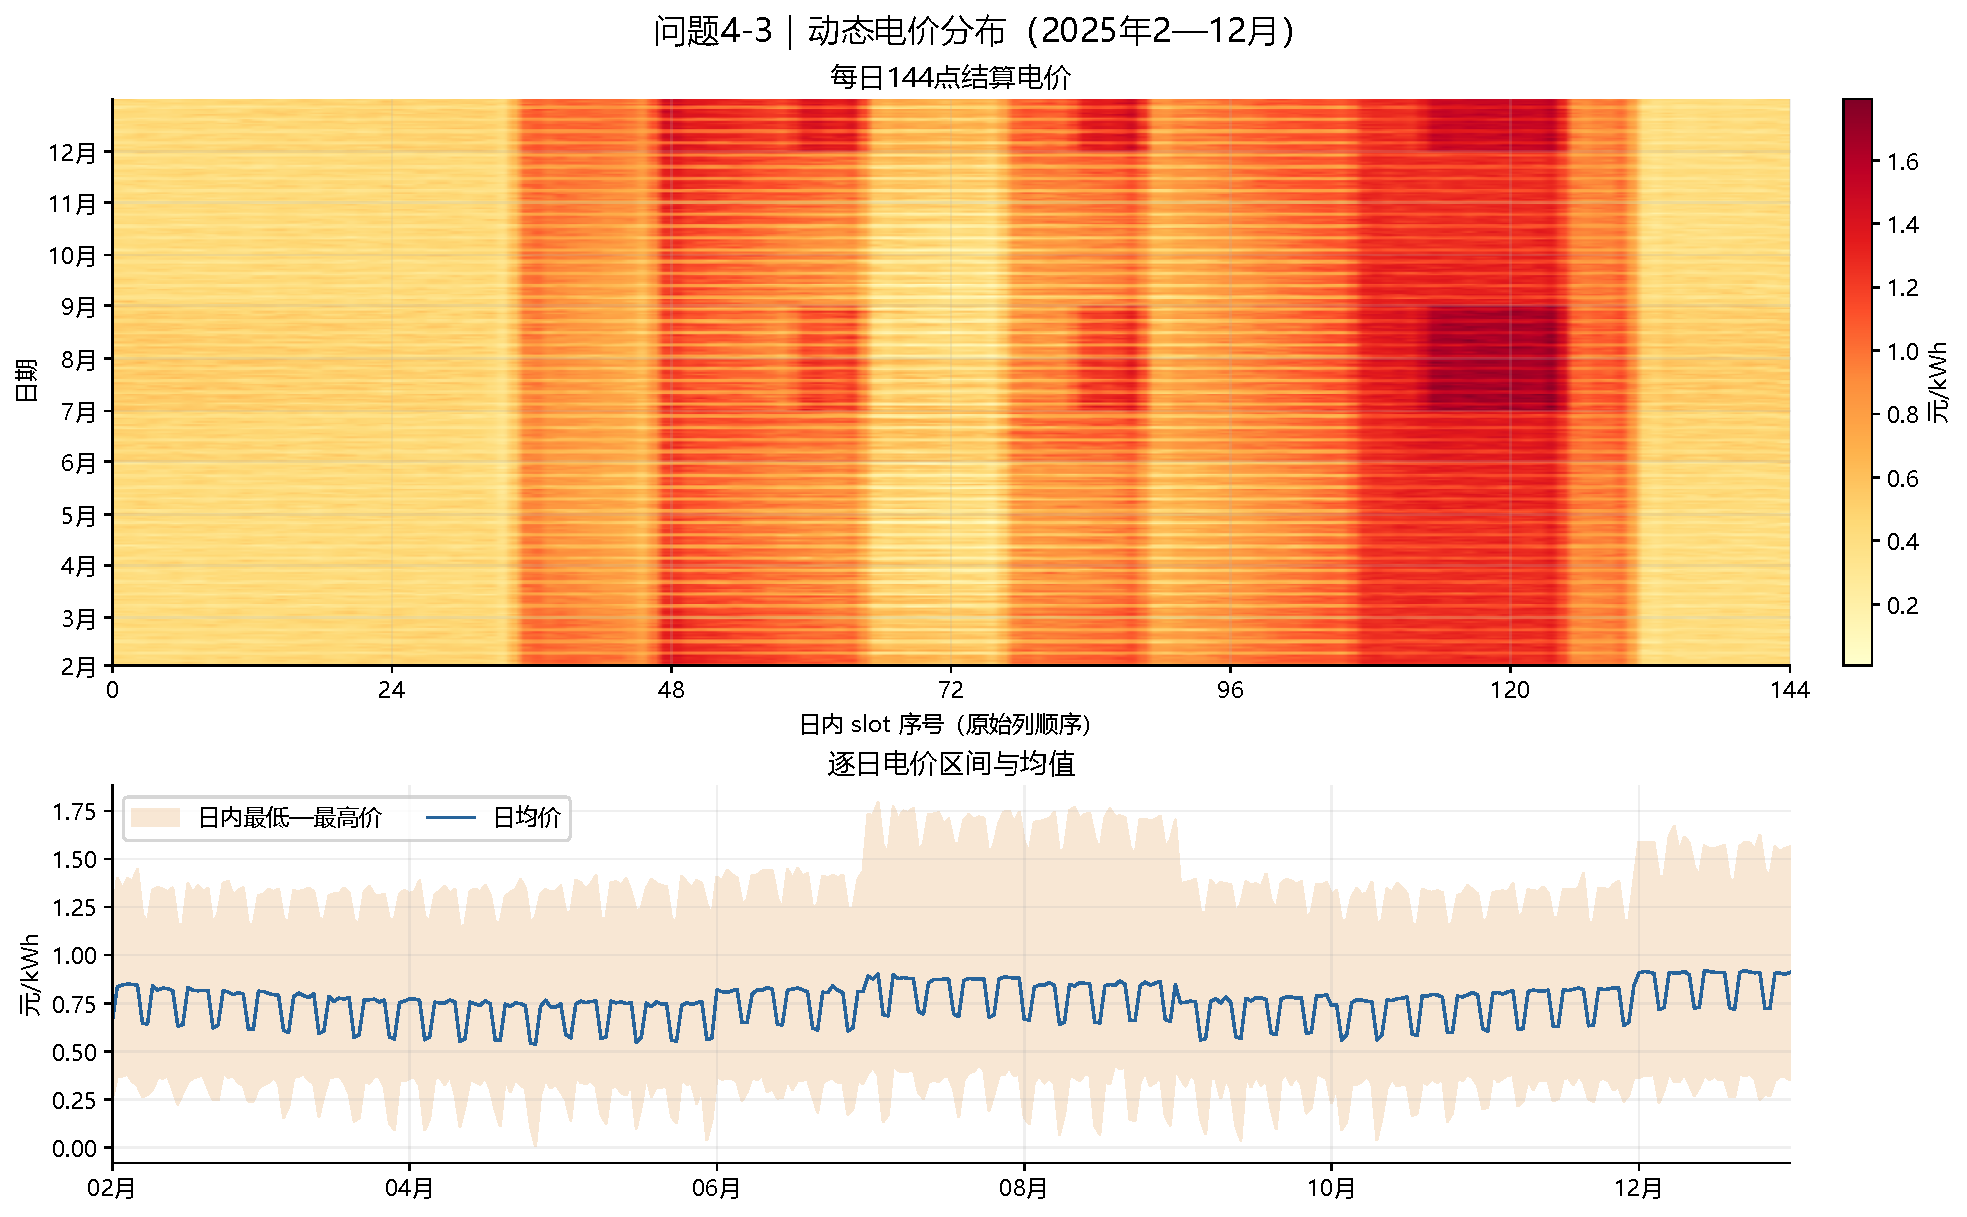
\includegraphics[width=.94\textwidth]{figures/q4_prices.pdf}
\caption{附件4的动态价格分布与日内波动特征}\end{figure}
4-3中价格峰谷差与储能吞吐量的描述性相关系数为-0.0299，未显示明显正相关。因此不能将“峰谷差越大必然充放电越多”写成当前数据结论。相关统计也不构成价格波动影响的因果识别。
\subsection{指定日期结果}
所有电量单位为kWh，费用单位为元，保留四位小数，总量使用未舍入值计算。指定十分钟区间按模板标签查询，时间口径见前文。
\Needspace{140pt}\begingroup\centering\captionof{table}{问题4-2：指定时段购电及全天合同费用}\fontsize{9}{11}\selectfont\setlength{\tabcolsep}{2pt}\renewcommand{\arraystretch}{1.13}
\noindent\begin{minipage}{\textwidth}\centering\textbf{2025-03-20}\par\smallskip
\begin{tabularx}{\textwidth}{|Y|Y|Y|Y|Y|Y|}\hline 时间段&购电量&时间段&购电量&时间段&购电量\\\hline
10:00-10:10 & 0.0000 & 12:00-12:10 & 671.0825 & 14:00-14:10 & 0.0000\\\hline
16:00-16:10 & 545.0921 & 18:00-18:10 & 715.8517 & 20:00-20:10 & 729.7183\\\hline
\multicolumn{2}{|c|}{全天合同购电量}&76140.7317&\multicolumn{2}{c|}{全天合同购电费}&47497.6864\\\hline\end{tabularx}\end{minipage}\par\medskip
\noindent\begin{minipage}{\textwidth}\centering\textbf{2025-06-21}\par\smallskip
\begin{tabularx}{\textwidth}{|Y|Y|Y|Y|Y|Y|}\hline 时间段&购电量&时间段&购电量&时间段&购电量\\\hline
10:00-10:10 & 0.0000 & 12:00-12:10 & 735.1763 & 14:00-14:10 & 0.0000\\\hline
16:00-16:10 & 524.8433 & 18:00-18:10 & 701.5525 & 20:00-20:10 & 888.2017\\\hline
\multicolumn{2}{|c|}{全天合同购电量}&77616.4592&\multicolumn{2}{c|}{全天合同购电费}&38449.1099\\\hline\end{tabularx}\end{minipage}\par\medskip
\noindent\begin{minipage}{\textwidth}\centering\textbf{2025-09-23}\par\smallskip
\begin{tabularx}{\textwidth}{|Y|Y|Y|Y|Y|Y|}\hline 时间段&购电量&时间段&购电量&时间段&购电量\\\hline
10:00-10:10 & 0.0000 & 12:00-12:10 & 494.2704 & 14:00-14:10 & 0.0000\\\hline
16:00-16:10 & 457.1233 & 18:00-18:10 & 802.0687 & 20:00-20:10 & 508.3743\\\hline
\multicolumn{2}{|c|}{全天合同购电量}&68909.8634&\multicolumn{2}{c|}{全天合同购电费}&44029.5706\\\hline\end{tabularx}\end{minipage}\par\medskip
\noindent\begin{minipage}{\textwidth}\centering\textbf{2025-12-21}\par\smallskip
\begin{tabularx}{\textwidth}{|Y|Y|Y|Y|Y|Y|}\hline 时间段&购电量&时间段&购电量&时间段&购电量\\\hline
10:00-10:10 & 0.0000 & 12:00-12:10 & 910.9646 & 14:00-14:10 & 0.0000\\\hline
16:00-16:10 & 778.8025 & 18:00-18:10 & 727.5967 & 20:00-20:10 & 0.0000\\\hline
\multicolumn{2}{|c|}{全天合同购电量}&93437.8248&\multicolumn{2}{c|}{全天合同购电费}&69304.3080\\\hline\end{tabularx}\end{minipage}\par\medskip
\raggedright 注：购电量为日前计划，合同费用不含紧急购电费。\par\endgroup\medskip
\Needspace{140pt}\begingroup\centering\captionof{table}{问题4-2：指定时段储能充放电及首末储电量}\fontsize{9}{11}\selectfont\setlength{\tabcolsep}{2pt}\renewcommand{\arraystretch}{1.12}
\noindent\begin{minipage}{\textwidth}\centering\textbf{2025-03-20}\par\smallskip\begin{tabularx}{\textwidth}{|Y|Y|Y|Y|Y|Y|}\hline 时间段&充电量&放电量&时间段&充电量&放电量\\\hline
0:00-4:00 & 2000.0000 & 0.0000 & 4:00-8:00 & 4166.6667 & 4772.4051\\\hline
8:00-12:00 & 5850.7628 & 4542.5949 & 12:00-16:00 & 5919.3802 & 893.8158\\\hline
16:00-20:00 & 0.0000 & 6442.3836 & 20:00-24:00 & 5333.3333 & 2197.6164\\\hline
\multicolumn{2}{|c|}{0:00储电量}&6000.0000&\multicolumn{2}{c|}{24:00储电量}&6000.0000\\\hline\end{tabularx}\end{minipage}\par\medskip
\noindent\begin{minipage}{\textwidth}\centering\textbf{2025-06-21}\par\smallskip\begin{tabularx}{\textwidth}{|Y|Y|Y|Y|Y|Y|}\hline 时间段&充电量&放电量&时间段&充电量&放电量\\\hline
0:00-4:00 & 833.3333 & 1345.2267 & 4:00-8:00 & 6204.7848 & 4974.9353\\\hline
8:00-12:00 & 5866.5994 & 3187.6593 & 12:00-16:00 & 6129.3106 & 1589.7416\\\hline
16:00-20:00 & 0.0000 & 5810.8187 & 20:00-24:00 & 5333.3333 & 2829.1812\\\hline
\multicolumn{2}{|c|}{0:00储电量}&6000.0000&\multicolumn{2}{c|}{24:00储电量}&6000.0000\\\hline\end{tabularx}\end{minipage}\par\medskip
\noindent\begin{minipage}{\textwidth}\centering\textbf{2025-09-23}\par\smallskip\begin{tabularx}{\textwidth}{|Y|Y|Y|Y|Y|Y|}\hline 时间段&充电量&放电量&时间段&充电量&放电量\\\hline
0:00-4:00 & 2833.3333 & 0.0000 & 4:00-8:00 & 2500.0000 & 6584.5173\\\hline
8:00-12:00 & 5484.0361 & 2055.4827 & 12:00-16:00 & 5442.4853 & 210.4823\\\hline
16:00-20:00 & 0.0000 & 6973.3333 & 20:00-24:00 & 5333.3333 & 1666.6667\\\hline
\multicolumn{2}{|c|}{0:00储电量}&6000.0000&\multicolumn{2}{c|}{24:00储电量}&6000.0000\\\hline\end{tabularx}\end{minipage}\par\medskip
\noindent\begin{minipage}{\textwidth}\centering\textbf{2025-12-21}\par\smallskip\begin{tabularx}{\textwidth}{|Y|Y|Y|Y|Y|Y|}\hline 时间段&充电量&放电量&时间段&充电量&放电量\\\hline
0:00-4:00 & 5333.3333 & 0.0000 & 4:00-8:00 & 833.3333 & 1508.3333\\\hline
8:00-12:00 & 5833.3333 & 7806.6667 & 12:00-16:00 & 7500.0000 & 2315.3528\\\hline
16:00-20:00 & 191.7936 & 5131.2538 & 20:00-24:00 & 5333.3333 & 3508.7462\\\hline
\multicolumn{2}{|c|}{0:00储电量}&6000.0000&\multicolumn{2}{c|}{24:00储电量}&6000.0000\\\hline\end{tabularx}\end{minipage}\par\medskip
\raggedright 注：四小时内充放电均为正表示不同十分钟时段的累计，不表示同时充放电。\par\endgroup
\begin{table}[H]\centering\caption{问题4-2：四个指定日期的紧急购电区间}\label{tab:emergency-问题4-2}\fontsize{9}{11}\selectfont\setlength{\tabcolsep}{2pt}\begin{tabular}{|lr|lr|lr|lr|}\hline
\multicolumn{2}{|c|}{2025-03-20} & \multicolumn{2}{|c|}{2025-06-21} & \multicolumn{2}{|c|}{2025-09-23} & \multicolumn{2}{|c|}{2025-12-21}\\\hline
时间段&购电量&时间段&购电量&时间段&购电量&时间段&购电量\\\hline
0:30-0:50 & 37.4563 & 无 & 0.0000 & 2:10-2:20 & 0.8426 & 0:10-0:20 & 3.3265\\
1:20-1:30 & 11.5129 &  &  & 6:10-8:10 & 490.6818 & 1:10-1:30 & 22.4663\\
18:10-18:30 & 8.8068 &  &  & 8:30-8:40 & 6.7917 & 1:40-1:50 & 1.5754\\
18:50-19:20 & 68.9363 &  &  & 9:30-11:20 & 520.6356 & 2:20-2:30 & 6.5004\\
20:10-20:30 & 53.6129 &  &  & 14:30-15:40 & 382.7140 & 3:10-3:30 & 59.6043\\
21:30-21:40 & 8.8117 &  &  & 16:00-18:00 & 370.6423 & 3:40-4:00 & 98.1948\\
23:40-23:50 & 24.6080 &  &  & 20:20-20:40 & 7.5098 & 4:20-4:30 & 0.1398\\
 &  &  &  & 21:00-21:10 & 9.3900 & 5:10-5:30 & 9.6256\\
 &  &  &  & 22:30-22:40 & 16.1867 & 5:40-6:10 & 47.7728\\
 &  &  &  &  &  & 6:20-6:40 & 25.1715\\
 &  &  &  &  &  & 7:0-7:20 & 10.0867\\
 &  &  &  &  &  & 7:50-8:10 & 24.5775\\
 &  &  &  &  &  & 8:30-8:50 & 39.6960\\
 &  &  &  &  &  & 9:00-9:20 & 26.6807\\
 &  &  &  &  &  & 9:40-10:00 & 33.1458\\
 &  &  &  &  &  & 10:30-12:00 & 1038.4861\\
 &  &  &  &  &  & 12:10-12:30 & 25.4431\\
 &  &  &  &  &  & 12:40-13:30 & 166.5758\\
 &  &  &  &  &  & 14:50-16:10 & 179.9651\\
 &  &  &  &  &  & 16:30-16:40 & 9.4271\\
 &  &  &  &  &  & 17:30-17:40 & 17.9450\\
 &  &  &  &  &  & 18:20-18:30 & 6.9191\\
 &  &  &  &  &  & 18:40-19:10 & 29.1800\\
 &  &  &  &  &  & 19:30-19:40 & 1.0733\\
 &  &  &  &  &  & 19:50-20:20 & 69.4854\\
 &  &  &  &  &  & 22:00-22:10 & 15.0150\\
 &  &  &  &  &  & 23:00-23:20 & 15.7499\\
 &  &  &  &  &  & 23:50-0:00+1 & 6.6598\\
\hline\end{tabular}\end{table}

\begin{table}[H]\centering\small
\caption{问题4-2：实际总购电与费用}
\begin{tabular}{lrrrr}\toprule
日期 & 实际购电量 & 紧急购电量 & 紧急费用 & 实际总费用\\\midrule
2025-03-20 & 76354.4766 & 213.7449 & 1045.3672 & 48543.0536\\
2025-06-21 & 77616.4592 & 0.0000 & 0.0000 & 38449.1099\\
2025-09-23 & 70715.2578 & 1805.3944 & 7981.0571 & 52010.6277\\
2025-12-21 & 95428.3138 & 1990.4890 & 9118.8195 & 78423.1274\\
\bottomrule\end{tabular}\end{table}
\FloatBarrier
\subsection{指定日期结果}
所有电量单位为kWh，费用单位为元，保留四位小数，总量使用未舍入值计算。指定十分钟区间按模板标签查询，时间口径见前文。
\Needspace{140pt}\begingroup\centering\captionof{table}{问题4-3：指定时段购电及全天合同费用}\fontsize{9}{11}\selectfont\setlength{\tabcolsep}{2pt}\renewcommand{\arraystretch}{1.13}
\noindent\begin{minipage}{\textwidth}\centering\textbf{2025-03-20}\par\smallskip
\begin{tabularx}{\textwidth}{|Y|Y|Y|Y|Y|Y|}\hline 时间段&购电量&时间段&购电量&时间段&购电量\\\hline
10:00-10:10 & \shortstack{0.0000\\0.0000} & 12:00-12:10 & \shortstack{599.0619\\521.3555} & 14:00-14:10 & \shortstack{0.0000\\0.0000}\\\hline
16:00-16:10 & \shortstack{646.6018\\493.7743} & 18:00-18:10 & \shortstack{711.7617\\711.7617} & 20:00-20:10 & \shortstack{729.7183\\729.7183}\\\hline
\multicolumn{2}{|c|}{全天合同购电量}&\shortstack{73540.3073\\68104.3475}&\multicolumn{2}{c|}{全天合同购电费}&\shortstack{45498.3173\\44219.9049}\\\hline\end{tabularx}\end{minipage}\par\medskip
\noindent\begin{minipage}{\textwidth}\centering\textbf{2025-06-21}\par\smallskip
\begin{tabularx}{\textwidth}{|Y|Y|Y|Y|Y|Y|}\hline 时间段&购电量&时间段&购电量&时间段&购电量\\\hline
10:00-10:10 & \shortstack{0.0000\\0.0000} & 12:00-12:10 & \shortstack{561.4173\\561.4173} & 14:00-14:10 & \shortstack{0.0000\\0.0000}\\\hline
16:00-16:10 & \shortstack{575.5241\\575.5241} & 18:00-18:10 & \shortstack{686.7649\\686.7649} & 20:00-20:10 & \shortstack{888.2017\\888.2017}\\\hline
\multicolumn{2}{|c|}{全天合同购电量}&\shortstack{74926.2075\\74783.7930}&\multicolumn{2}{c|}{全天合同购电费}&\shortstack{37486.1181\\37518.1788}\\\hline\end{tabularx}\end{minipage}\par\medskip
\noindent\begin{minipage}{\textwidth}\centering\textbf{2025-09-23}\par\smallskip
\begin{tabularx}{\textwidth}{|Y|Y|Y|Y|Y|Y|}\hline 时间段&购电量&时间段&购电量&时间段&购电量\\\hline
10:00-10:10 & \shortstack{0.0000\\0.0000} & 12:00-12:10 & \shortstack{445.1351\\430.5782} & 14:00-14:10 & \shortstack{23.4920\\0.0000}\\\hline
16:00-16:10 & \shortstack{600.6055\\563.8344} & 18:00-18:10 & \shortstack{833.5750\\833.5750} & 20:00-20:10 & \shortstack{519.1183\\519.1183}\\\hline
\multicolumn{2}{|c|}{全天合同购电量}&\shortstack{76310.5609\\74782.7314}&\multicolumn{2}{c|}{全天合同购电费}&\shortstack{49557.9160\\49078.6917}\\\hline\end{tabularx}\end{minipage}\par\medskip
\noindent\begin{minipage}{\textwidth}\centering\textbf{2025-12-21}\par\smallskip
\begin{tabularx}{\textwidth}{|Y|Y|Y|Y|Y|Y|}\hline 时间段&购电量&时间段&购电量&时间段&购电量\\\hline
10:00-10:10 & \shortstack{0.0000\\0.0000} & 12:00-12:10 & \shortstack{972.1554\\866.2299} & 14:00-14:10 & \shortstack{0.0000\\0.0000}\\\hline
16:00-16:10 & \shortstack{825.5984\\825.5984} & 18:00-18:10 & \shortstack{727.5967\\727.5967} & 20:00-20:10 & \shortstack{0.0000\\0.0000}\\\hline
\multicolumn{2}{|c|}{全天合同购电量}&\shortstack{95616.1888\\94807.1114}&\multicolumn{2}{c|}{全天合同购电费}&\shortstack{71384.8537\\71267.4193}\\\hline\end{tabularx}\end{minipage}\par\medskip
\raggedright 注：每格上行为0:00计划，下行为执行合同；下行合同费用为初始计划费加逐次调整净费。\par\endgroup\medskip
\Needspace{140pt}\begingroup\centering\captionof{table}{问题4-3：指定时段储能充放电及首末储电量}\fontsize{9}{11}\selectfont\setlength{\tabcolsep}{2pt}\renewcommand{\arraystretch}{1.12}
\noindent\begin{minipage}{\textwidth}\centering\textbf{2025-03-20}\par\smallskip\begin{tabularx}{\textwidth}{|Y|Y|Y|Y|Y|Y|}\hline 时间段&充电量&放电量&时间段&充电量&放电量\\\hline
0:00-4:00 & 2000.0000 & 0.0000 & 4:00-8:00 & 3333.3333 & 6001.7220\\\hline
8:00-12:00 & 5493.2105 & 2638.2780 & 12:00-16:00 & 5469.1180 & 244.7150\\\hline
16:00-20:00 & 21.2974 & 6454.7379 & 20:00-24:00 & 5333.3333 & 2197.2840\\\hline
\multicolumn{2}{|c|}{0:00储电量}&6000.0000&\multicolumn{2}{c|}{24:00储电量}&6000.0000\\\hline\end{tabularx}\end{minipage}\par\medskip
\noindent\begin{minipage}{\textwidth}\centering\textbf{2025-06-21}\par\smallskip\begin{tabularx}{\textwidth}{|Y|Y|Y|Y|Y|Y|}\hline 时间段&充电量&放电量&时间段&充电量&放电量\\\hline
0:00-4:00 & 833.3333 & 1345.2267 & 4:00-8:00 & 6301.4782 & 4835.8011\\\hline
8:00-12:00 & 5668.5263 & 3272.8270 & 12:00-16:00 & 5611.2061 & 1300.5077\\\hline
16:00-20:00 & 195.7802 & 5823.2065 & 20:00-24:00 & 5333.3333 & 2816.7935\\\hline
\multicolumn{2}{|c|}{0:00储电量}&6000.0000&\multicolumn{2}{c|}{24:00储电量}&6000.0000\\\hline\end{tabularx}\end{minipage}\par\medskip
\noindent\begin{minipage}{\textwidth}\centering\textbf{2025-09-23}\par\smallskip\begin{tabularx}{\textwidth}{|Y|Y|Y|Y|Y|Y|}\hline 时间段&充电量&放电量&时间段&充电量&放电量\\\hline
0:00-4:00 & 2833.3333 & 0.0000 & 4:00-8:00 & 2500.0000 & 6097.8774\\\hline
8:00-12:00 & 5893.1650 & 2517.5563 & 12:00-16:00 & 5663.8446 & 745.7440\\\hline
16:00-20:00 & 7.0598 & 6979.0518 & 20:00-24:00 & 5333.3333 & 1666.6667\\\hline
\multicolumn{2}{|c|}{0:00储电量}&6000.0000&\multicolumn{2}{c|}{24:00储电量}&6000.0000\\\hline\end{tabularx}\end{minipage}\par\medskip
\noindent\begin{minipage}{\textwidth}\centering\textbf{2025-12-21}\par\smallskip\begin{tabularx}{\textwidth}{|Y|Y|Y|Y|Y|Y|}\hline 时间段&充电量&放电量&时间段&充电量&放电量\\\hline
0:00-4:00 & 5333.3333 & 0.0000 & 4:00-8:00 & 833.3333 & 1656.5123\\\hline
8:00-12:00 & 5833.3333 & 7403.0251 & 12:00-16:00 & 7365.6197 & 2633.6307\\\hline
16:00-20:00 & 356.2915 & 5118.8381 & 20:00-24:00 & 5333.3333 & 3482.7419\\\hline
\multicolumn{2}{|c|}{0:00储电量}&6000.0000&\multicolumn{2}{c|}{24:00储电量}&6000.0000\\\hline\end{tabularx}\end{minipage}\par\medskip
\raggedright 注：四小时内充放电均为正表示不同十分钟时段的累计，不表示同时充放电。\par\endgroup
\begin{table}[H]\centering\caption{问题4-3：四个指定日期的紧急购电区间}\label{tab:emergency-问题4-3}\fontsize{9}{11}\selectfont\setlength{\tabcolsep}{2pt}\begin{tabular}{|lr|lr|lr|lr|}\hline
\multicolumn{2}{|c|}{2025-03-20} & \multicolumn{2}{|c|}{2025-06-21} & \multicolumn{2}{|c|}{2025-09-23} & \multicolumn{2}{|c|}{2025-12-21}\\\hline
时间段&购电量&时间段&购电量&时间段&购电量&时间段&购电量\\\hline
0:30-0:50 & 37.4563 & 无 & 0.0000 & 2:10-2:20 & 0.8426 & 0:10-0:20 & 3.3265\\
1:20-1:30 & 11.5129 &  &  & 20:20-20:40 & 7.5098 & 1:10-1:30 & 22.4663\\
8:20-8:40 & 28.2239 &  &  & 21:00-21:10 & 9.3900 & 1:40-1:50 & 1.5754\\
8:50-9:30 & 137.5983 &  &  & 22:30-22:40 & 16.1867 & 2:20-2:30 & 6.5004\\
9:50-10:10 & 57.9445 &  &  &  &  & 3:10-3:30 & 59.6043\\
11:10-12:10 & 345.6128 &  &  &  &  & 3:40-4:00 & 98.1948\\
12:40-13:00 & 150.4760 &  &  &  &  & 4:20-4:30 & 0.1398\\
13:10-13:50 & 148.0535 &  &  &  &  & 5:10-5:30 & 9.6256\\
14:00-14:40 & 40.9799 &  &  &  &  & 5:40-6:10 & 47.7728\\
15:30-16:30 & 93.3849 &  &  &  &  & 6:30-6:40 & 0.4267\\
16:40-17:00 & 5.1731 &  &  &  &  & 8:00-8:10 & 13.3395\\
18:10-18:30 & 8.8068 &  &  &  &  & 8:30-8:40 & 6.0161\\
18:50-19:20 & 71.7835 &  &  &  &  & 9:00-9:10 & 0.7455\\
20:10-20:30 & 53.6129 &  &  &  &  & 9:40-10:10 & 57.1657\\
21:30-21:40 & 8.8117 &  &  &  &  & 10:30-10:40 & 30.1744\\
23:40-23:50 & 24.6080 &  &  &  &  & 10:50-12:30 & 651.1456\\
 &  &  &  &  &  & 12:50-13:20 & 99.6146\\
 &  &  &  &  &  & 17:30-17:40 & 17.9450\\
 &  &  &  &  &  & 18:20-18:30 & 6.9191\\
 &  &  &  &  &  & 18:40-19:10 & 30.7700\\
 &  &  &  &  &  & 19:30-19:40 & 2.4650\\
 &  &  &  &  &  & 19:50-20:20 & 84.0870\\
 &  &  &  &  &  & 22:00-22:10 & 15.0150\\
 &  &  &  &  &  & 23:00-23:20 & 15.7499\\
 &  &  &  &  &  & 23:50-0:00+1 & 6.6598\\
\hline\end{tabular}\end{table}

\begin{table}[H]\centering\small
\caption{问题4-3：实际总购电与费用}
\begin{tabular}{lrrrr}\toprule
日期 & 实际购电量 & 紧急购电量 & 紧急费用 & 实际总费用\\\midrule
2025-03-20 & 69328.3866 & 1224.0390 & 4936.1720 & 49156.0769\\
2025-06-21 & 74783.7930 & 0.0000 & 0.0000 & 37518.1788\\
2025-09-23 & 74816.6604 & 33.9290 & 139.0167 & 49217.7084\\
2025-12-21 & 96094.5564 & 1287.4449 & 5561.4233 & 76828.8427\\
\bottomrule\end{tabular}\end{table}
\FloatBarrier

\begin{figure}[H]\centering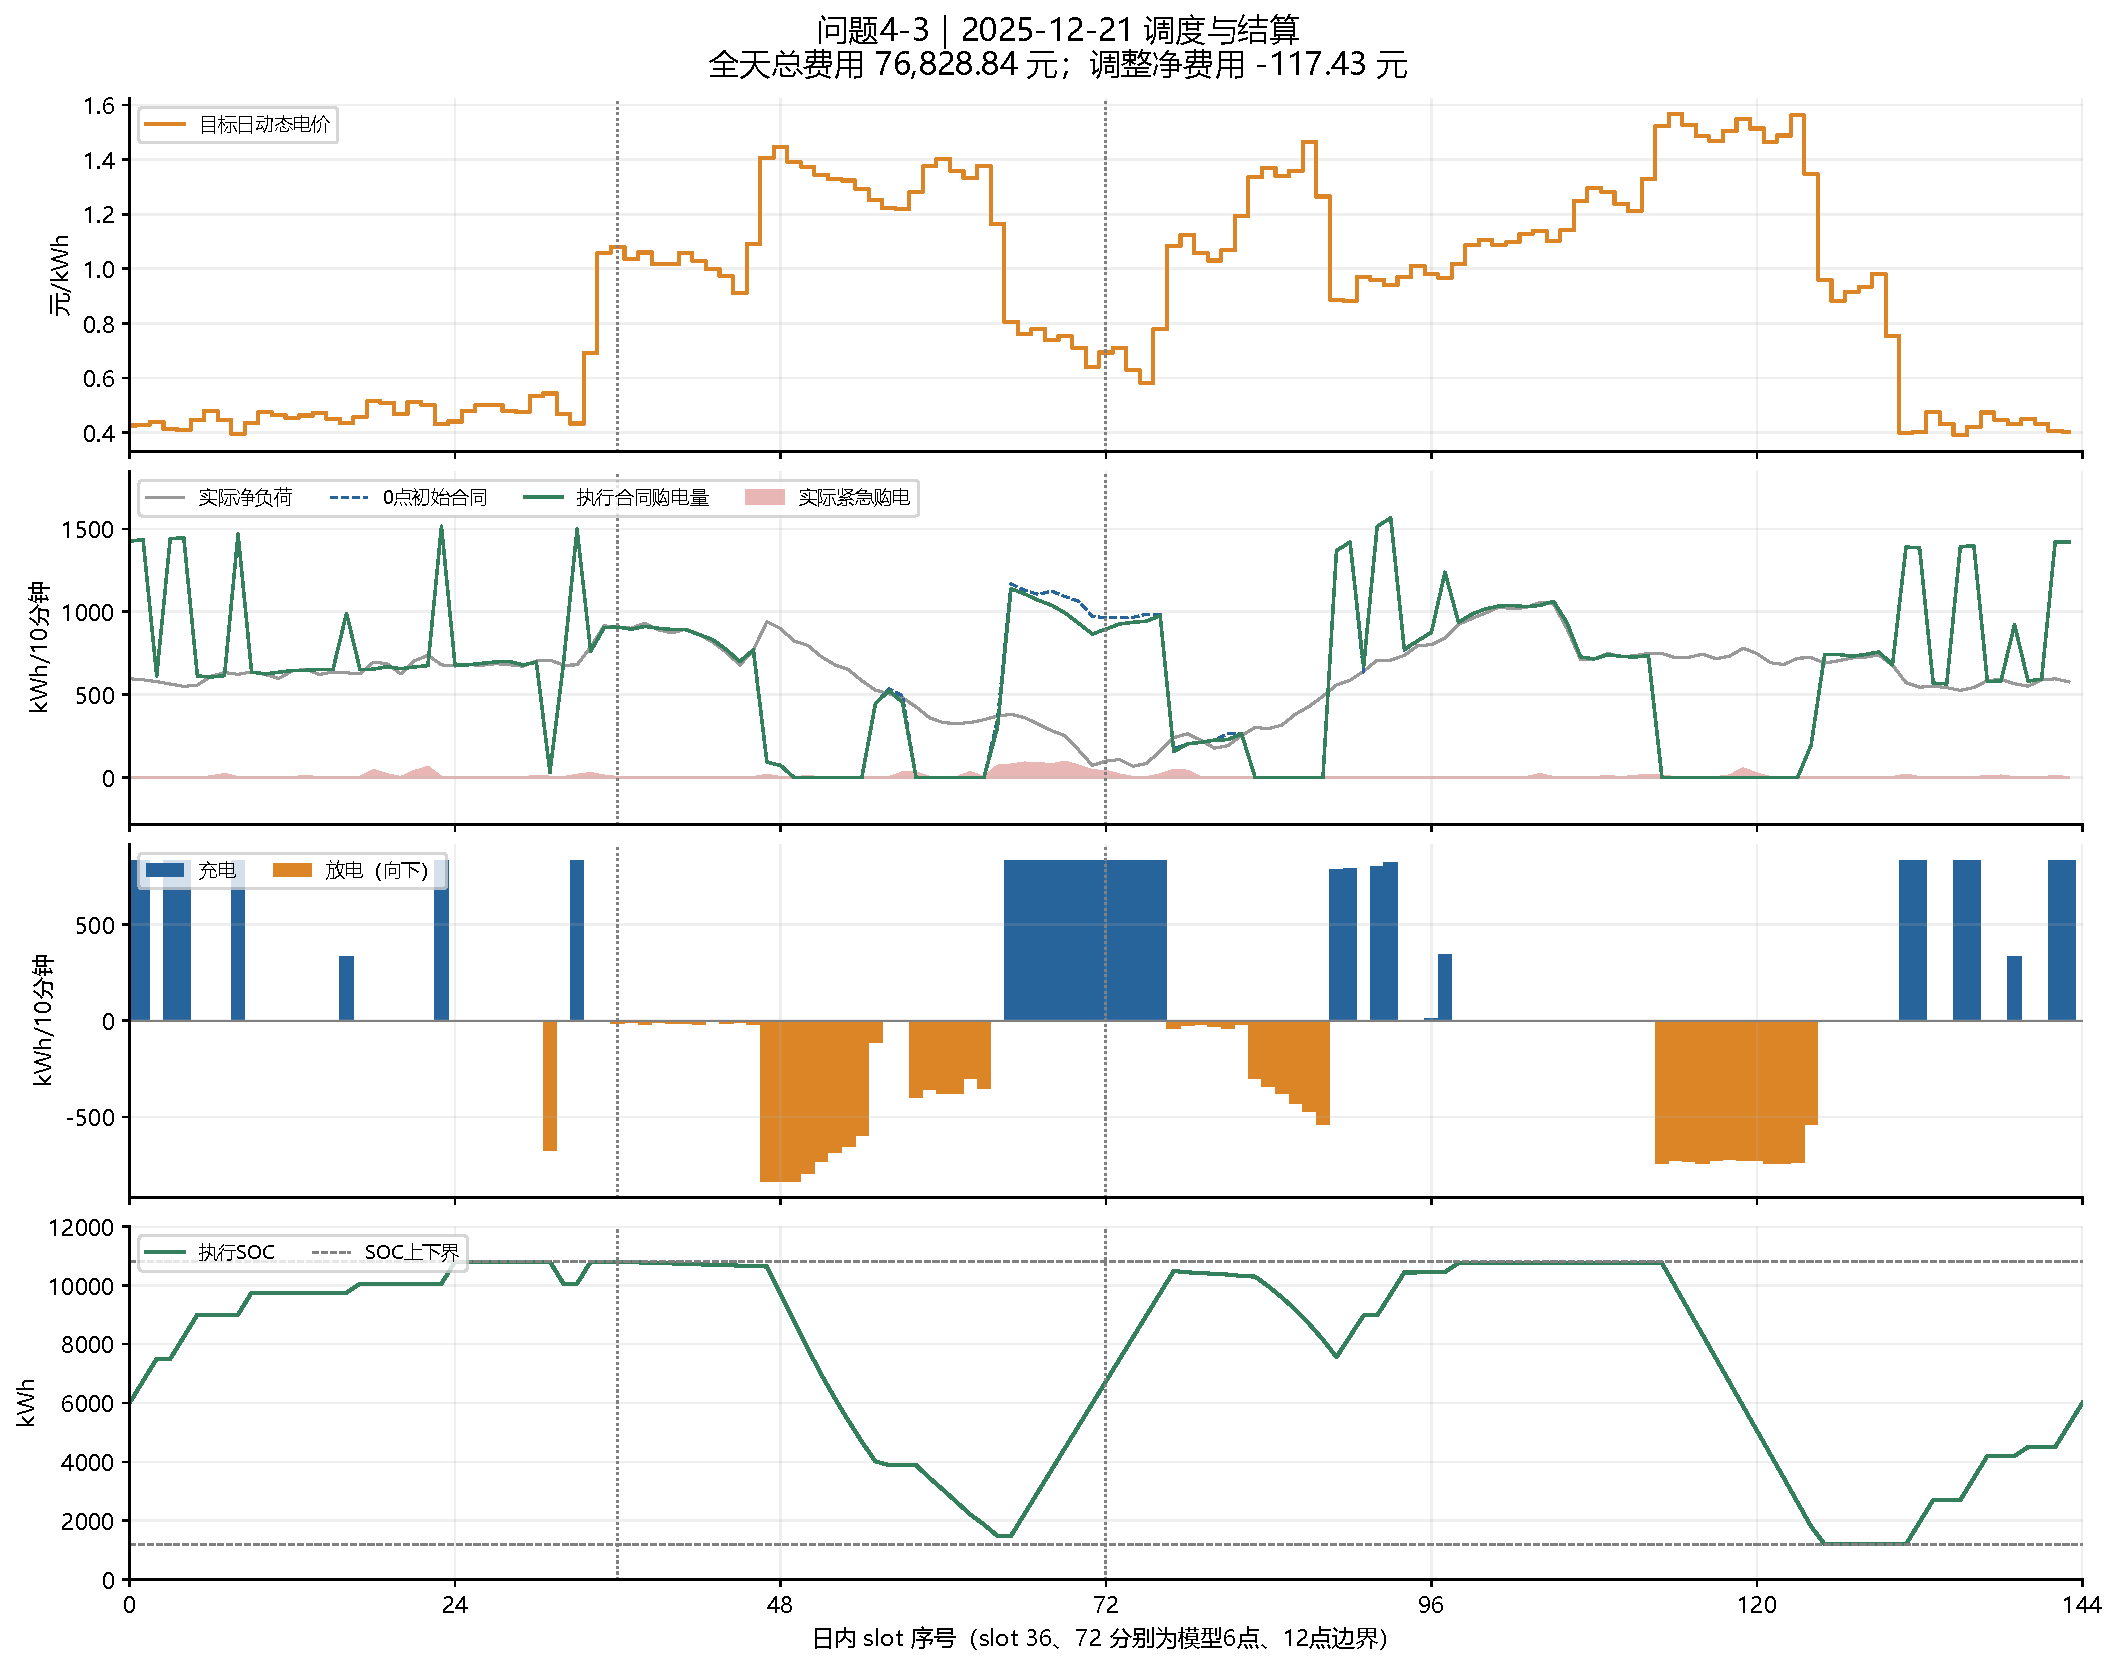
\includegraphics[width=.94\textwidth]{figures/q4_dispatch.pdf}
\caption{波动价格下12月21日的滚动合同与储能执行策略}\end{figure}
\FloatBarrier
